\documentclass{hbrs-ecta-report}
\usepackage{float}
\usepackage{placeins}
\usepackage{ngerman}
%\usepackage[utf8]{inputenc}
\usepackage{fontspec}
\begin{document}

\conferenceinfo{H-BRS}{2017}

\title{Neuroevolution: NeuroEvolution of Augmenting Topologies (NEAT)}
\subtitle{}

\numberofauthors{2}
\author{
\alignauthor
Tim L"ugger, Jan Urfei
}

\date{today}
\maketitle
\begin{abstract}
Aufgabe: Implementieren Sie NEAT auf den Herzfrequenz Daten. Bestimmen Sie die besten Hyperparameter. Wiederholen Sie ihr Experiment 10 mal und vergleichen Sie die Ergebnisse mit den Ergebnissen aus ESP bezogen auf die Zeit und den Fehler.
Plottet die durchschnittliche Elite, die Elite und den durchschnittlichen Median über alle Experimente.
Außerdem plotte die Anzahl an Knoten und Kanten über die Generationen.
\end{abstract}

\section{Herangehensweise}
\subsection{Aufbau}
 Das Erste, was wir uns überlegt haben ist, wie wir eine Topologie repräsentieren. Grundlegend haben wir zwei Listen, eine für die Knoten in einem Netz und eine für die Verbindungen (siehe Figure \ref{fig:Genomtabelle}). Das Ganze wird intern als Matrix abgespeichert, um besser damit rechnen zu können. Deswegen haben wir bei den Knoten auch den Typ in Zahlen codiert. 1 Steht für einen Input-, 2 für einen Hidden- und 3 für einen Outputknoten. Bei den Kanten steht die 1 für enabled und die 0 für disabled.
 \begin{figure}[h!]
 	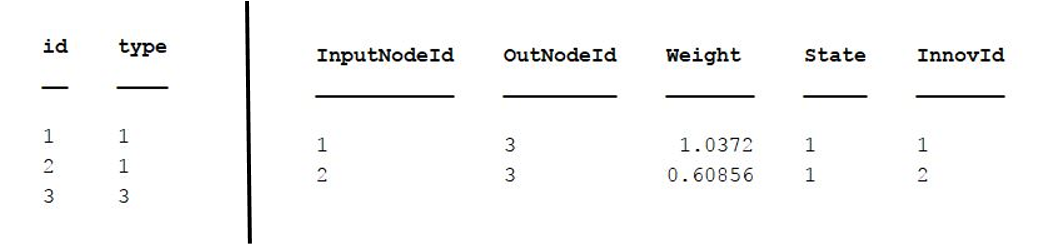
\includegraphics[width=\linewidth]{img/Genomtabelle}
 	\caption{Repräsentation eines Genoms. Links für die Knoten und rechts für die Kanten}
 	\label{fig:Genomtabelle}
 \end{figure}

Mit der Datei phenotyp.m lassen wir die Gewichtsmatrix aus den zwei oben genannten Matrizen erzeugen. Diese ist genauso aufgebaut wie die, die wir im ESP verwendet haben.\\

Als nächstes haben wir die Funktionen implementiert, die für die Mutation bzw. für den Crossover gebraucht werden. Die appendNode und addConnection hängen einfach nur weitere Zeilen in die in Figure \ref{fig:Genomtabelle} gezeigte Liste. Wenn Kannten hinzugefügt wird muss allerdings noch überprüft werden, ob in der gleichen Iteration schon einmal zufällig eine gleiche Innovation stattgefunden hat und wenn ja muss diese nämlich die gleiche Innovationsid bekommen. Im Zuge der Mutationen haben wir auch Funktionen geschrieben, die Kanten enablen, disablen oder switchen. Nicht alle der drei Funktionen werden im Moment verwendet, aber sie sind schon einmal da, damit spätere Erweiterungen einfacher werden.\\ 
Die Funktion mutateAdd arbeitet wie in der Vorlesung und dem Paper beschrieben. Sie erstellt einen neuen Knoten und hängt diesen zwischen zwei, wobei die alte Kante disabled wird und die eine neue Kante das Kantengewicht 1 und die andere das der alten Kante bekommt.
Die MutateAddConnection fügt eine noch nicht vorhande Kante hinzu. Dafür werden 4 zufällige Kanten erzeugt und geguckt ob eine davon noch nicht existiert. Wenn es alle schon gibt passiert nichts.
Die Funktion mutateWeights implementiert das, was in den bisherigen Algorithmen eigentlich nur gemacht wurde, und zwar die Kantengewichte anzupassen. Dazu werden zu 90 Prozent aller Kanten ein normalverteilter Zufallswert addiert. Wie viel Prozent verändert werden klären wir in Kapitel \ref{sec:parameter}. Der Crossover ist genau so umgesetzt, wie im Paper beschrieben.\\

Was dann noch fehlt ist eine Methode, die die Distanz zwischen zwei Netzen bestimmt, um diese nachher einer Spezies zuordnen zu können. Diese bekommt zwei Knotenlisten übergeben und muss dann erst einmal bestimmen welche die kleinere ist um diese durchgehen zu können. Die erste Liste wird also durchgegangen und bei jeder Kante wird geguckt ob sie gleich zur anderen Liste ist, disjunkt oder extra vorkommt. Je nachdem werden die Parameter E,D und W erhöht. Da es vorkommen kann, dass die zweite Liste auch Kanten hat, die in der ersten nicht vorkommen, muss ich mir die bis dorthin abgehandelten Kanten markieren und iteriere in einem zweiten Schritt noch über die nicht behandelten Kanten. Am Ende muss das Gewicht noch gemittelt werden, wie es das Paper verlangt und die Distanz mit Hilfe der Funktion $ \dfrac{c1*E}{N}+\dfrac{c2*D}{N}+c3*\bar{W}$ bestimmt werden.\\

Mit Hilfe von dieser Funktion können jetzt die Spezies eingeteilt werden. Dazu wird die erste Topologie in eine eigene Spezies gepackt. Danach wird über alle drüber iteriert und geguckt ob die Distanz unter einem gewissen Schwellwert liegt (Kapitel \ref{sec:parameter}). Wenn ja bekommt sie die gleiche Spezies wenn nicht wird eine neue eröffnet. Die Spezies werden in einem Vektor abgespeichert, indem der erste Wert für die Spezies des ersten Netzes steht. Wenn der Zielwert an Spezies nicht erreicht oder übertroffen wird, verändert sich auch der Schwellwert, für die nächste Berechnung.\\

Wie eingangs schon erwähnt wird die Berechnung des Ergebnisses eines Netzes ähnlich wie beim ESP durchgeführt, da ja auch Rekurrenz theoretisch entstehen kann. Das führt allerdings dazu, dass wenn keine direkte Kante vom Input zum Output führt das Ergebnis verzögert ist. \\

Die Methode FitnessCalulation berechnet für alle Netze die Fitness. Dafür wird pro Netz über alle Trainingszeitreihen nacheinander gegangen und der Fehler aufsummiert. Die Aktivierung von einem Netz wird nach jeder Zeitreihe aber wieder auf den Startzugang zurück gesetzt.\\

In unserem Hauptprogramm werden dann alle Funktionen im Prinzip sinnvoll hintereinander aufgerufen. Nach erstellen einer Startpopulation werden erst die Spezies bestimmt und dann die Fitness für alle berechnet. Danach sortieren wir die Population und werfen die schlechtesten raus. Für den genauen Anteil verweise ich wieder auf Kapitel \ref{sec:parameter}. Im folgenden werden die Eliten von Spezies, die mehr als 5 groß sind unverändert übernommen. Dafür suchen wir die Indizes dieser uns speichern diese. Als nächstes wird die aktuelle Größe der Population abgespeichert und die Entfernten Topologien mittels Crossover wieder aufgefüllt. Als letztes werden über die nicht Elite Topologien bis zu den neu aufgefüllten iteriert und mit einer gewissen Wahrscheinlichkeit mutiert. Der ganze Ablauf ist in Figure \ref{fig:Ablauf} nochmals grafisch dargestellt.\\
 \begin{figure}[b!]
	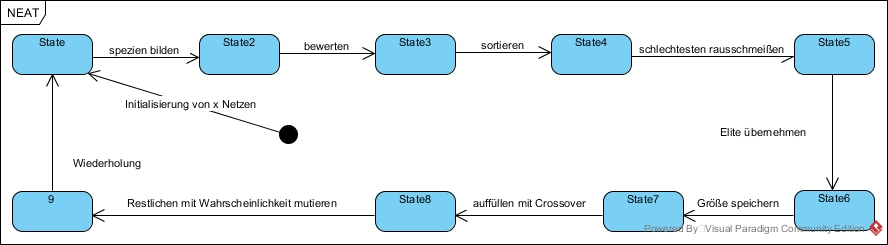
\includegraphics[width=2\linewidth]{img/Ablauf}
	\caption{Ablauf uneseres NEAT Algorithmus}
	\label{fig:Ablauf}
\end{figure}

Der komplette Verlauf des Projektes mit den einzelnen Schritten kann auch auf unserem GitHub Repository (\url{https://github.com/timlueg/Neuroevolution/commits/master}) nachvollzogen werden. \\ 

\subsection{Hyperparameter}\label{sec:parameter}
Zu der Anzahl an Topologien innerhalb von NEAT lässt sich sagen, dass mit 150 Topologien bei gleicher Anzahl an Generationen bessere Ergebnisse erzielt werden (siehe Figure \ref{fig:150Topos} im Vergleich zu Figure \ref{fig:NeatElite}). Mit 150 Topologien dauert die Berechung aber erheblich länger. Sinnvoller ist es daher
 die Anzahl an Topologien etwas kleiner zu wählen und dafür die Anzahl an Generationen zu erhöhen.\\
\begin{figure}[h!]
	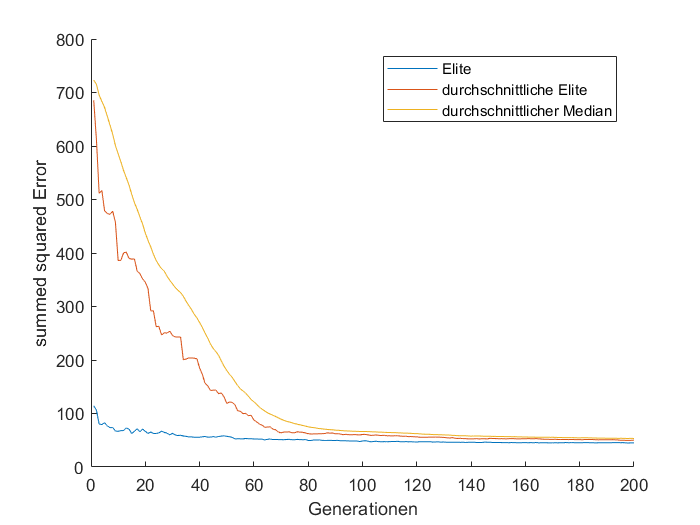
\includegraphics[width=\linewidth]{img/150Topos}
	\caption{2 Experimente worüber pro Iteration der Durchschnitt bzw. der Beste genommen wurde}
	\label{fig:150Topos}
\end{figure}

Die Gewichte (c1,c2,c3) für die Distanzfunktion haben wir aus dem Paper übernommen. Für die Distanz zwischen den Spezies haben wir festgestellt, dass die die ersten Iterationen immer bis unter 0.5 absinkt, weswegen wir diese initial auf 0.3 setzen und dafür die Schritte, mit denen angepasst wird, wenn das Target nicht erreicht wird auf 0.05 gesetzt haben.\\

Die Wahrscheinlichkeit, dass ein Netz mutiert wird beträgt 80\% und ist auch aus dem Paper entnommen, genauso wie die Wahrscheinlichkeit dass eine Kante innerhalb eines Netzes mutiert wird 90\% beträgt und die restlichen 10\% ein zufälliges Gewicht gesetzt wird. Die Standardabweichung mit der die Gewichte verändert werden ist nur 0.04. Das erschien uns sinnvoll, da die meisten Gewichte in Intervall $[-1;1]$ liegen und so die Änderungen nur hinreichend klein sind.
\newpage
\section{Unsere Ergebnisse}
\subsection{NeatErgebnisse}
Man kann in Figure \ref{fig:NeatElite} sehen, dass die Populationen, die keinen günstigen Start haben sich sehr schnell anpassen können. Auch ohne den Crossover lassen sich schon ganz gute Werte erzielen.\\
\begin{figure}[h!]
	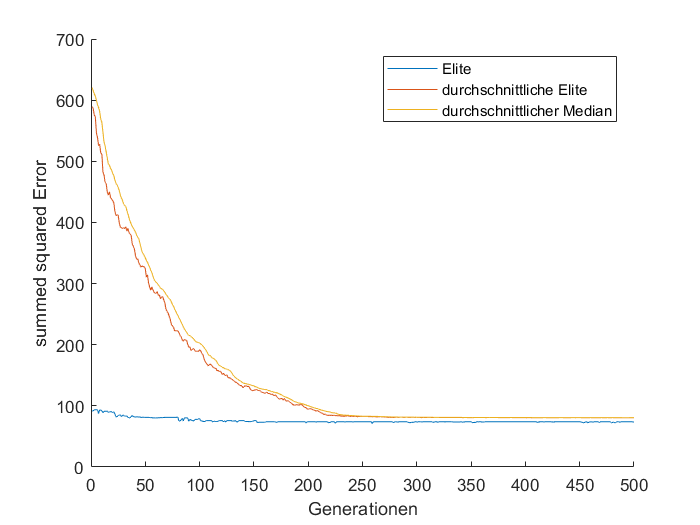
\includegraphics[width=\linewidth]{img/NeatElite}
	\caption{10 Experimente worüber pro Iteration der Durchschnitt bzw. der Beste genommen wurde}
	\label{fig:NeatElite}
\end{figure}

Figure \ref{fig:KantenUndKnoten} lässt erkennen, dass die Kanten deutlich zunehmen, im Gegensatz zu der Anzahl an Knoten. Daraus lässt sich schließen, dass sich tendenziell eher Netze mit einem hohen Grad an Vermaschung ergeben, was auch den Aussagen der Vorlesung entspricht, da für eine Zeitreihenvorhersage Netze mit Rekurrenz besser geeignet sind.\\
\begin{figure}[h!]
	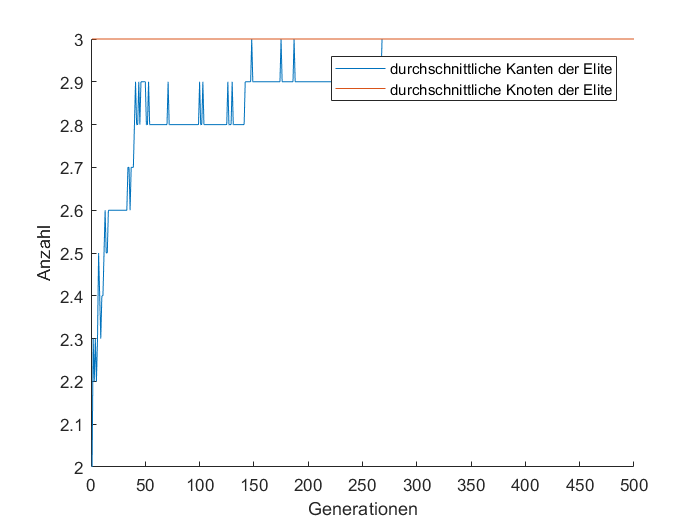
\includegraphics[width=\linewidth]{img/KantenUndKnoten}
	\caption{Die gemittelte Anzahl an Knoten und Kanten über 10 Experimente}
	\label{fig:KantenUndKnoten}
\end{figure}

Unsere Anzahl an Topologien sind über die Generationen hinweg immer größer oder gleich der Zahl die wir anfangs gesetzt haben (siehe Figure \ref{fig:VerlaufTopo}). Das liegt daran, dass wir diese Zahl, nachdem wir die ''schlechten'' rausgeschmissen haben, mit crossover wieder auffüllen, dabei können auch etwas mehr entstehen, als die ursprüngliche Anzahl.\\
\begin{figure}[h!]
	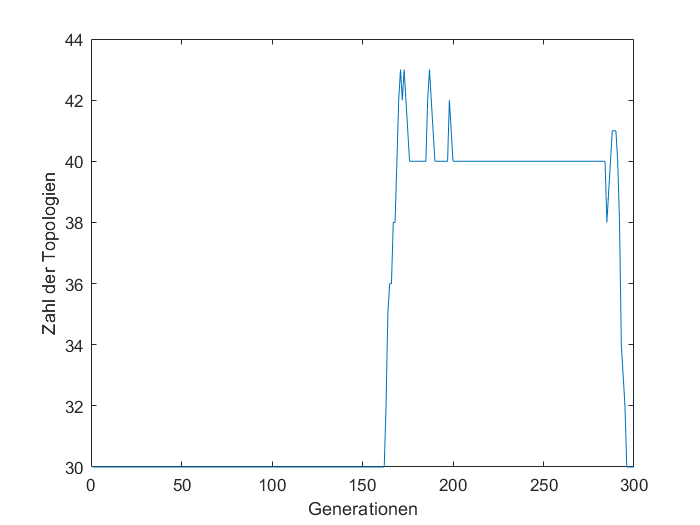
\includegraphics[width=\linewidth]{img/VerlaufTopo}
	\caption{Verlauf der beinhalteten Topologien}
	\label{fig:VerlaufTopo}
\end{figure}

Nach 300 Iterationen sieht ein Netz, welches die Fitness 46 hat z.B. aus wie das Netz was in Figure \ref{fig:BeispielTopologie}. Die Knoten, die nicht erreicht werden können, bzw. von denen es kein Weg zum Output gibt sind orange eingefärbt.


\subsection{Verlgeich zu ESP}
Im Vergleich zu ESP (Figure \ref{fig:ESP}) sieht man, dass der Fehler viel höher anfängt, da sich Rekurrenz, die für die Vorhersage einer Zeitreihe notwendig ist bei NEAT erst mit der Zeit bildet. Bei ESP ist sie von vorne herein gegeben, da wir ein vollvermaschtes Netz vorgeben.\\
\begin{figure}[h!]
	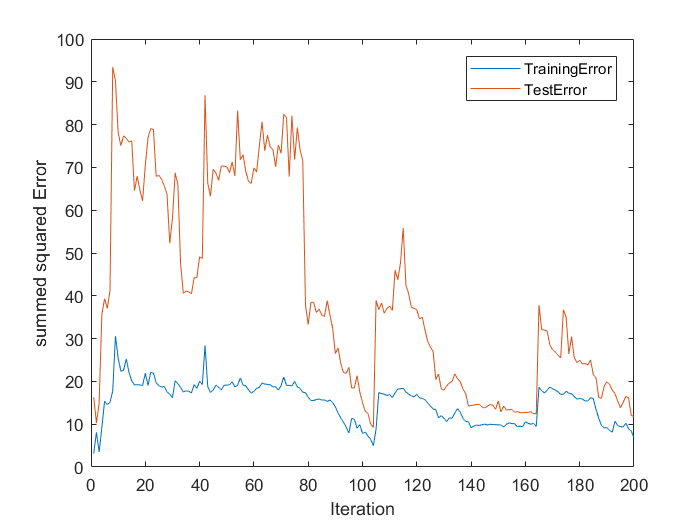
\includegraphics[width=\linewidth]{img/ESP2}
	\caption{Der Trainings- und Testerror über 200 Generationen}
	\label{fig:ESP}
\end{figure}
\newpage
\begin{figure}[t!]
	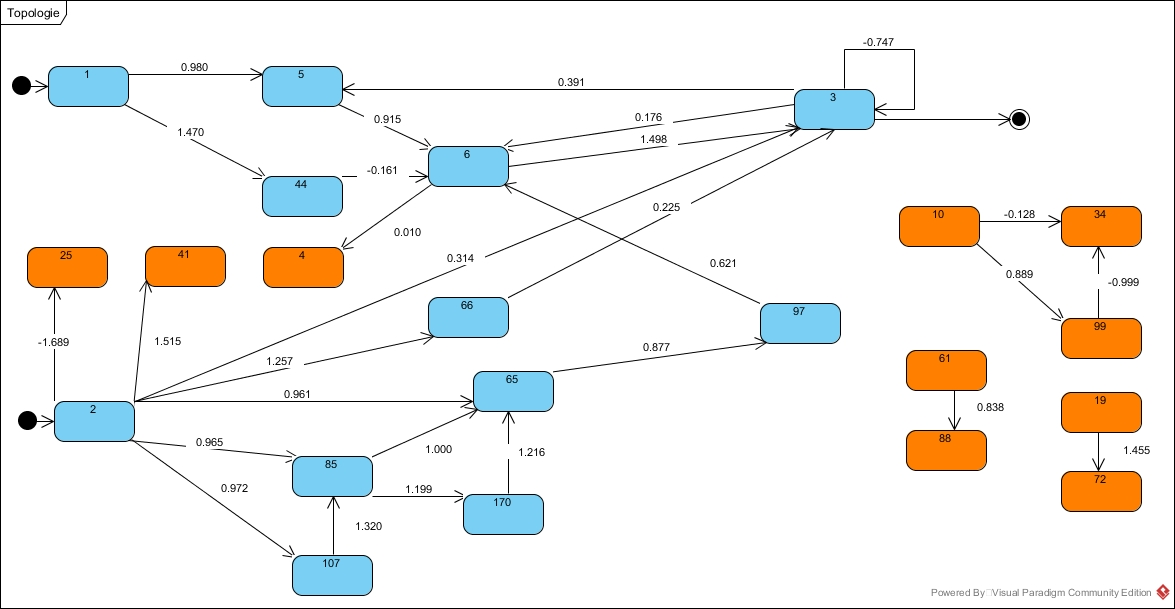
\includegraphics[width=2\linewidth]{img/BeispielTopologie}
	\caption{bestes Netz nach 300 Generationen}
	\label{fig:BeispielTopologie}
\end{figure}

Der Fehlerwert an sich ist leider nicht direkt vergleichbar, da bei NEAT der Fehler über alle Zeitreihen aufsummiert wird. Beim ESP wird der Fehler nur nach jeder einzelnen Zeitreihe berechnet, da dann die Gewichte angepasst werden. Ganz grob kann man die Fehler vergleichen, wenn man den Fehler vom NEAT durch 10 teilt, da der Fehler über 10 mal so viele Zeitreihen aufsummiert wird. Ganz genau stimmt das dennoch leider nicht.\\
Aber was die Konvergenz betrifft kann man sagen, dass der ESP Algorithmus nach 200 Generationen noch nicht konvergiert. In Figure \ref{fig:NeatElite} ist aber erkennbar, dass es bei NEAT schon ab 130 Generationen zur konvergenz kommt.\\



\section{Offene Baustellen}
Aktuell ist die Gewichtsmartix der Netze noch sehr unoptimiert aufgebaut, sodass das ausführen von Netzen bei großer Knotenzahl sehr lange dauert und damit unsere Auswertung sehr aufwendig ist.
Weiterhin wurde fitness Sharing vorerst nicht implementiert sondern allen Spezies die gleiche Anzahl an Offspring aus Crossover erlaubt. Außerdem wird Crossover immer auf alle Spezies >= 2 angewandt und die Parents beibehalten (aber mutiert).
Nicht geklärt ist weiterhin, ob es vorteilhaft ist, eine Population (< Größe der Startpopulation) mit Mutationen aufzufüllen bis mindestens die Größe der Startpopulation erreicht ist.


\end{document}
}